
\begin{abstract}
% XXX one paragraph limit

% XXX changed "score" to "selection"
We propose a nonparametric procedure to achieve fast inference in generative graphical models when the number of latent states is very large.
 The approach is based on iterative latent variable preselection, where we alternate between learning a 'selection function' to reveal the relevant latent variables, and use this to obtain a compact approximation of the posterior distribution for EM; this can make inference possible where the number of possible latent states is e.g. exponential in the number of latent variables, whereas an exact approach would be computationally unfeasible.
We learn the selection function entirely from the observed data and current EM state via Gaussian process regression: this is by contrast with earlier approaches, where selections were hand-designed for each problem setting.
We show our approach to perform as well as these bespoke selection functions on a wide variety of inference problems: in particular, for the challenging case of a hierarchical model for object localization with occlusion, we achieve results that match a customized state-of-the-art selection method,  at a far lower computational cost.






%Specifically, for the preselection step, a computationally efficient selection function is used to select the relevant latent variables from the full set, given an observation. This preselected set is then used to represent the posterior distribution with reduced support.
%TODO
\end{abstract}

% XXX 8 pages text + references
% - Citations within the text should include the author's last name and year, e.g., (Cheesman, 1985).
% - Be sure that the sentence reads correctly if the citation is deleted
% - Make sure that the figure caption does not get separated from the figure.

\section{Introduction}
%
%TODO
%- Embed work in Landscape of Sexiness (TM)\\
%- Discuss new stuff from Welling, old stuff... \\
%- mention leverage score relation\\
%- Take some ideas from abstract



Inference in probabilistic graphical models can be challenging in situations where
there are a large number of hidden variables, each of which may take on one of several
state values. The EM algorithm is widely applied for inference when hidden variables
are present, however inference can quickly become intractable as the dimensionality increases.

More general grounding of motivation, before get into more specific general grounding?  I.e. challenges of big data / scaling and other shiny BS people love to hear, and how the simplest quick approach that can handle inference should be chosen, stuff from Bottou paper~\cite{Bottou08thetradeoffs} we somehow forgot to cite.


Expectation truncation (ET) \citep{LuckeEggert2010} is a meta algorithm for accelerating EM learning
in graphical models, which restricts the inference performed during the E-step
to an ``interesting'' subset of states of the latent variables,  %The subset is
chosen per data point according to a \emph{selection function}.
In previous work, functions to select states of high posterior mass were hand-crafted to model the properties of the graphical model of interest, using intuition from noiseless limits or upper-bound results specific to the model \citep{LuckeEggert2010,SheltonEtAl2012,BornscheinEtAl2013,SheikhEtAl2014}.
The crucial underlying assumption remains that the posterior mass is finally concentrated in small volumes of the latent state space.
%\footnote{Approaches using sparse priors (i.e. automatic relevance determination (ARD) prior) find sparse subsets of states across all observations in a final model, whereas ours provides relevant features for each observation (often different between observations), to guide EM iterations towards regions of high posterior probability in any model.}
% (a property exploited by earlier ET approaches).
This property is observed to hold in many visual data and general pattern recognition settings.

The general idea of aiding inference in graphical models by
learning a function that maps from the observed data to
a property of the latent variables is quite old, dating back at least to the
Helmholtz machine and its bottom-up connections trained using the wake-sleep
algorithm \citep{HintonEtAl1995}.
More recently, the idea has surfaced in the context of learning variational distributions with neural networks~\citep{WellingICML2014}.
A two-stage inference has furthermore been discussed in the context of
computer vision \citep{YuilleKersten2006} and neural inference \citep{KoernerEtAl1999}.
Recently, researchers~\citep{MnihGregor2014} %http://jmlr.org/proceedings/papers/v32/mnih14.pdf
have generalized this idea to learning in arbitrary graphical models by training
an ``inference network'' that efficiently implements sampling from the posterior
distribution.

For more complex graphical models, notably the hierarchical model of \citep{DaiLucke2014},  the design of suitable selection functions
is extremely challenging: it requires both expert knowledge
on the problem domain and considerable computational resources to implement
 (indeed, the design of such functions for  particular problems
has been a major contribution in several of the foregoing papers).

In the present work, we propose a generalization of the ET approach, where
we avoid completely the challenge of problem-specific selection function design.
Instead,
we learn this function  adaptively and nonparametrically
from the data,
 while learning the model
parameters  simultaneously using EM.
We emphasize that the selection function is  used only to ``guide'' the underlying
base inference algorithm to regions of high posterior probability, but is not itself
used as an approximation to the posterior distribution. As such, the learned
function does not have to be a completely accurate indication of latent
variable predictivity,
as long as the relative importance of states is preserved.
We use  Gaussian process
regression \citep{RasmussenGPbook} to learn the selection function, though other regression techniques could
also be applied. The main advantage of GPs
is that they have an analytic one-shot learning procedure, and that learning different
functions based on the same inputs is computationally cheap, which makes adaptive learning
of a changing target function efficient. We term this part of our approach
\textit{GP-selection}.
Our nonparametric generalization of  ET may be applied as a black-box
meta algorithm for accelerating inference in  generative graphical models,
with no expert knowledge required.




%Can probably add some more here if needed


We have applied GP-selection in a number of experimental benchmarks.
First, we considered the case of sparse coding models (binary sparse coding,
spike-and-slab, nonlinear spike-and-slab), where the relationship between the
observed and latent variables is known to be complex and nonlinear.\footnote{Note that
 even
when linear relations exist between the latents and outputs, a nonlinear
regression may still be necessary in finding relevant variables,
as a result of explaining away.}
We show that GP-selection can produce results with equal performance to the respective  hand-picked selection functions.
Interestingly,
we find it can be essential to use nonlinear GP regression
in the spike-and-slab case, and that simple linear regression is not
sufficiently flexible in modelling the posterior shape.
Second, we illustrate GP-selection on a simple Gaussian mixture
model,
where we explicitly show the form of the learned regression function: this matches
well with our expectations for the model, and again reveals that it may be essential
to learn a nonlinear mapping.
Finally, we present results
for a recently published hierarchical model for  translation invariant occlusion components analysis
\citep{DaiLucke2014}.
The performance of our inference algorithm matched that of the complex
hand-engineered selection function of the previous work, while being straightforward
to implement and having a far lower computational cost.

%on a recent translation-invariant model, showing the ability of our approach to
%successfully do inference in a sophisticated hierarchical model -- with
%performance matching that of the model's complex hand-engineered selection
%function -- and while being applicable to larger scale problems.
%In these experiments, Gibbs sampling from the reduced latent space lead to further decrease computational costs.
%Furthermore, we show that with this approach we can do inference in challenging models and scale to a large number of latent variables.


\section{Variable selection for accelerated inference}
\label{method}
%
\textbf{Notation.}
%Notation throughout the paper will be as follows.
We denote the observed data by the matrix $\vec{Y}=(\vec{y}^{(1)}, \dots, \vec{y}^{(N)})$, where each vector $\vec{y}^{(n)} = ( y_1^{(n)}, \dots, y_D^{(n)})^\mathrm{T}$ is the $n$th observation 
in a $D$-dimensional space.
Similarly we define corresponding 
binary latent variables\footnote{We restrict ourselves to binary latent variables here, though
discrete variables with higher cardinality can easily be used by
converting them into binary variables.} 
by the matrix $\vec{S} = (\vec{s}^{(1)}, \dots, \vec{s}^{(N)})\in \{0,1\}^{N \times H}$ 
where each $\vec{s}^{(n)}=(s_1^{(n)}\dots, s^{(n)}_H)^\mathrm{T} \in \{0,1\}^{H}$ is the $n$th vector in the $H$-dimensional latent space,
and for each individual hidden variable $h$, the vector $\vec{s}_h=(s_h^{(1)}\dots, s^{(N)}_h)\in \{0,1\}^{N}$. 
%
We denote the prior distribution over the latent variables with $p(\vec{s} | \theta)$ 
and the likelihood of the data with $p(\vec{y} | \vec{s}, \theta)$
% TODO check wording here
Using these expressions, the posteror distribution over latent variables is 
%
\vspace{-.2cm}
\begin{equation}
\label{eq:post}
p(\vec{s}^{(n)}|\vec{y}^{(n)},\Theta)  = \frac{p(\vec{s} | \theta) \, p(\vec{y} | \vec{s}, \theta)}
{\disS\hspace{-1.5mm}\sum_{\vec{s}\Prime^{(n)}} p(\vec{s} | \theta) \, p(\vec{y} | \vec{s}, \theta)}.
\end{equation}

\subsection{Expectation Maximization}
Expectation Maximization (EM) is an iterative algorithm to optimize the model parameters of a given graphical model.
EM iteratively optimizes a lower bound on the data likelihood by inferring the
posterior distribution over hidden variables given the current parameters (the
E-step), and then adjusts the parameters to maximize the likelihood of the
data averaged over this posterior (the M-step).
%
When the number of latent states to consider is large (e.g.\ exponential in the
number of latent variables), the computation of the posterior distribution in
the E-step becomes intractable and approximations are required.

%(also, depending on the model at hand, it can suffice to compute the
%expectations of some functions of the latent variables with respect to the
%posterior, such as the expected latent mean or variance).
%
% From JL: Note that Zhenwen's y entries are not necessarily in R. Also corrected s notation.
%

\subsection{Selection with Expectation Truncation}
%%%%%%%%%%%%%%%%%%
% Describe how ET works, how it relates to EM. An inference algorithm that takes $\Kn$ and gives you a $q$
%%%%%%%%%
%
Expectation truncation (ET) is an extension of the expectation maximization (EM) algorithm (e.g. \citep{DempsterEtAl1977,
NealHinton1998}).
%
The main idea underlying ET is that for a given observation $\vec{y}^{(n)}$
only a subset of the $H$ latent variables $s_h^{(n)}$ will be relevant, meaning
that the marginal posterior probability $p^{(n)}_h \equiv p(s^{(n)}_h = 1|\vec{y}^{(n)}, \Theta)$
exceeds some threshold. 
% TODO want some reference to a graphical nmodel here?
A selection function is used to identify this subset
of variables, which in turn is used to define a subset $\mathcal{K}_n$ of the space. 
Variables not in this set (non-relevant variables) are fixed to 0.
%
The posterior distribution~\eqref{eq:post} can then be approximated by a truncated posterior distribution, computed on reduced support:
%
%\small
\vspace{-.1cm}
\begin{align}
\label{eq:sel-post}
p(&\vec{s}^{(n)}|\vec{y}^{(n)},\Theta) \nonumber\\
&\approx q_n(\vec{s}^{(n)};\Theta) = \frac{p(\vec{s}^{(n)},\vec{y}^{(n)}|\,\Theta) \,\delta(\vec{s}^{(n)}\in\hspace{-.05mm}\Kn)}
   %{\ disS\hspace{-1.5mm}\int_{\vec{s}\Prime^{(n)}\in\mathcal{K}_n}\hspace{-8mm} p(\vec{s}\Prime^{(n)},\vec{y}^{(n)}|\,\Theta)\,d\vec{s}\Prime^{(n)}}
{\disS\hspace{-1.5mm}\sum_{\vec{s}\Prime^{(n)}\in\mathcal{K}_n}\hspace{-3mm} p(\vec{s}\Prime^{(n)},\vec{y}^{(n)}|\,\Theta)},
\end{align}
\normalsize
%\vspace{-.2cm}
%
where $\Kn$ contains the indices of relevant latent states for data point
$\vec{y}^{(n)}$, and $\delta(\vec{s}\in\mathcal{K}_n)=1$ if
$\vec{s}\in\mathcal{K}_n$ and zero otherwise.
Note that $\Kn$ is not an arbitrary set of the possible states, but is axis aligned according to the latent states that are zero, which is more challenging. \comment{Jan, what did you mean here?}
%FIXME 

%%%%
%Describe selection function in general, what it looks like and does, and define functions $f$, $\Ih$
%current 4 dif fthings relating to selection function
%first give a name to all of these components w/o GP
%
%define f--
%introduce new function, call it f takes data point $y^(n)$, produces ability, jointly oredicts probabiity of all latents being 1
%vector of each $s_h$ -- vector of f for each $y^n$
%(f is one step behind $f_h$, where $f_h$ takes data point and predicts the expected value of $s_h$ )
%take top K' values,
%3 step process
%S_h takes y^(n) and produces a K_n


\subsection{ET with affinity} % TODO can remove when structure is stand-alone
%%%%%%
One way of constructing a selection function $\mathcal{S}^{(n)}$ is by
ranking the latent variables according to an 
\emph{affinity function} $f_h(\vec{y}^{(n)}) : \mathrm{R}^D \mapsto \mathrm{R}^{+}$
which directly reflects the relevance of latent variable $s_h$. A natural choice
for such a function is one that approximates the marginal posterior probability,
e.g.\ we try to learn $f$ such that $f_h(\vec{y}^{(n)}) \approx p^{(n)}_h$.
%
% TODO FIXME
%THERE NEEDS TO BE A BIT MORE TEXT HERE TO LINK THESE TWO.
% ************ XXX -----------------------------------
When the $H$ latent variables in the marginal posterior probability $\vec{p} = p_{h=1}^{(n)},\dots, p_H^{(n)}$ are conditionally independent given a data point $\vec{y}^{(n)}$,  this affinity function correctly isolates the most relevant variables in the posterior.
%
Even when this strong assumption does not hold in practice, which is often the case, 
the affinity can still highlight relevant variables; 
it has been empirically shown to be quite effective when dependencies exist.

% TODO REMOVE REDUNANCY XXX
%XXX Using these concepts, we define a general selection function to isolate the relevant regions $\Kn$ as follows.
%First, we define $f_h(\vec{y}^{(n)})$ as a function that takes the input of a single data
%point $\vec{y}^{(n)}$ and predicts the probability that the latent variable
%$s_h$ is equal to $1$ for this particular data point, such that each data point
%$\vec{y}^{(n)}$ is associated with an $H$-dimensional vector of predictions
%$\vec{f}(\vec{y}^{(n)}) = (f_1(\vec{y}^{(n)}), \dots, f_H(\vec{y}^{(n)}))$.
%
Next, using all $p_{h=1}^{(n)},\dots, p_H^{(n)}$ approximated marginal posterior probabilities from the affinity function $\vec{f}(\vec{y}^{(n)})$, we define 
 $\gamma(\vec{p}^{(n)})$ to sort the indices in descending order and \textit{reduce} the sorted set to $H' << H$ 
To ensure that there is a non-zero probability of choosing each state per EM iteration, $10\%$ of the $H'$ indices are uniformly chosen at random.
%
%of the indices $I$ corresponding
%to the highest probability states that $\vec{s}^{(n)}=1$ 
(i.e. all $h=1,\dots,H'$ latent variables sorted by estimated relevance).
%s a function of each
%$\vec{s}^{(n)}$ that returns a sorted and reduced set of indices $I$ corresponding
%to the highest probability states that $\vec{s}^{(n)}=1$ (output from $\vec{f}(\vec{y}^{(n)})$).
%In other words, $\gamma(\vec{s}^{(n)})$
%sorts all $h,...,H$ of the $s_h^{(n)}$ variables in descending order of estimated relevance.
%
Finally, we define $\mathcal{I}(I)$ to return an $H'$-dimensional vector for each data point $\vec{y}^{(n)}$, containing the set of selected relevant latent states indices $\Kn$. 
All 'non-relevant' variables $h\not\in I$ are effectively set to $0$ in Equation~\eqref{eq:sel-post} 
by not being present in the state set $\Kn$.
%to $0$, and returns the set of $H'$ selected relevant latent states' indices $\Kn$.
% with the "non-relevant" variables set to $0$ ($\mathcal{K}_n = \{\vec{s}^{(n)}\,|\,\mbox{for all}\ h\not\in I:\ s_h=0 \}$).
%
%for $K_n$ ... $\mathcal{I}(s) = K_n$ takes a given I, makes $K_n$, basically
%what that math says, but a function that does it
%takes subset of the H variables, produces a subset where everything NOT in subset is set to 0 ... say where s comes from
%We define $\mathcal{K}_n$ as $\mathcal{K}_n = \{\vec{s}\,|\,\mbox{for all}\ h\not\in I:\ s_h=0 \}$ where $\mathcal{I}$ contains the indices of the latents estimated to be most relevant for $\vec{y}^{(n)}$.
%

Using $f_h$, $\Ih$ and $\gamma$, we can define a \emph{selection function}
$\mathcal{S}_h(\vec{y}^{(n)})$ to select subsets $\mathcal{K}_n$ per data point
$\vec{y}^{(n)}$, with the goal of containing most of the probability mass
$\prob{\vec{s}}{\vec{y}}$ while also being significantly smaller than the entire
latent space.  
%
The \textit{general selection function}  can be expressed as
%
\vspace{-.1cm}
\begin{equation}\label{eq:sel-func}
\mathcal{S}(\vec{y}^{(n)}) \;=\; \mathcal{I} \left[  \gamma \left[ \vec{f}(\vec{y}^{(n)}) \right]  \right] \;=\; \mathcal{K}_n.
\end{equation}
%
So far, the form of $\mathcal{S}_h(\vec{y}^{(n)})$ has been
a hand-engineered deterministic function derived based on the structure of the considered model
(see e.g. \citep{SheltonEtAl2011, SheltonEtAl2012, DaiLucke2012a, DaiLucke2012b,
BornscheinEtAl2013, SheikhEtAl2014}).

%Using such subsets $\mathcal{K}_n$, Equation~\eqref{eq:sel-post} results in good approximations to the full posteriors.
%redundant: When the set $\Kn$ fulfills the above property of containing the indices of the states with concentrated posterior mass, Equation~\eqref{eq:sel-post} is a good approximation of the full posterior.

\subsection{Inference in EM with selection}
%
As a meta-algorithm, ET selects the $\Kn$ subspace prior to every EM iteration.
In each iteration, $\Kn$ is used to approximate posterior distribution by calculating the true posterior on the truncated space, $q(\vec{s})$,
 with which inference can be performed using any standard method.
Potential examples are to perform exact inference or to draw Gibbs samples from $q(\vec{s})$ for a sampling approximation of the truncated posterior.

To summarize, in one iteration of this approximate EM algorithm, the following
occurs: prior to the E-step, the algorithm is given a latent variable subset
$\Kn$ computed by the selection function $\Sh$ to use in the E-step.  Based on
this, the E-step computes and returns the approximate posterior distribution
$q(\vec{s})$.  This result is then used to calculate the model parameter update
equations in the M-step.


\section{GP-Select}
%
%In this work we generalize the above approach, where instead of defining $\Sh$
%by hand, we propose that $\Sh$ be learned in a black-box fashion based on the
%data.
We now generalize this approximate EM algorithm:  %for inference in graphical models
instead of predefining the form of $\Sh$ for variable selection, we want
to learn it in a black-box and model-free way based on the data.
%
The case we consider is to learn $\Sh$ by using Gaussian process (GP) regression
(e.g. \citep{RasmussenGPbook}), which is flexible, can make exact predictions,
and scales cubicly with the number of data points $N$ but linearly with the number of latent variables $H$.  
%
%Thus, with the previously defined concepts, we can express the Gaussian process model for the posterior marginal probability that $s_h^{(n)}=1$:
%generative story for a single latent variable $s_h$ as:
%
% TODO REMOVE XXX
%\begin{align}\label{eq:gen-story}
%f_h(\vec{y}^{(n)}) \sim \text{GP}\left(0, \, k(\cdot,\cdot) \right), \,\,\,
%p_h^{(n)} \sim f(\vec{y}^{(n)}) + \epsilon^{(n)}, \\
%\text{and}\quad \epsilon^{(n)} \sim \mathcal{N}(0,\sigma^2_{noise})
%\end{align}
%
%
%TODO put in reasons GPs are awesome!! XXX 
Specifically, we will define the affinity function $f_h$ as being drawn from a Gaussian process model: 
$f_h(\vec{y}^{(n)}) \sim \text{GP}\left(0, \, k(\cdot,\cdot) \right)$, where $k(\cdot, \cdot)$ is the covariance kernel, which can flexibly govern the representation of the relationship between variables.
Again, we use $f_h$ to approximate the marginal posterior probability $p_h$ that $s_h^{(n)}=1$.
%
A nice property of Gaussian processes is that we only need to compute the kernel matrix $K$ once (until updating of it's hyperparameters) 
to approximate the marginal posterior probability for the entire $N\times H$ set of latent variables $\vec{S}$.

% DO NOT EVEN USE: and $\sigma_{noise}^2$ is the degree of Gaussian noise on the function $f_h$.
Thus, in each EM iteration, we calculate the affinity function by using a GP to regress $\vec{S}$ onto $\vec{Y}$.  
Specifically, we define our training data as the \textit{expectations} of latent variables $\vec{s}$ 
and the set of observed variables $\vec{Y}$, namely 
%$\mathcal{D} = \{ (\vec{y}^{(n)}, \langle\vec{s}_{\text{prev-it}}\rangle^{(n)}_{q(\vec{s})}) | n = 1,\dots, N \}$.
$\mathcal{D} = \{ (\vec{y}^{(n)}, \langle\vec{s}\rangle^{(n)}_{q(\vec{s})}) | n = 1,\dots, N \}$.
%
%output of the previous iteration of the % EM parameter inference algorithm, $q(\vec{S})$, or rather, the expectations of
%This means that in the very first EM iteration contains no actual information from the posterior distribution, and 
In the first EM iteration, the expectations $\langle\vec{s}\rangle^{(n)}_{q(\vec{s})}$ are initialized randomly, 
in each subsequent EM iteration, the true expecations w.r.t. the $\Kn-$truncated posterior $q(\vec{s})$ are used. 

% TODO details here why XXX
We do this because.... 
We compute the predictive mean for of the predictive probability defined by the GP regression model \comment{(???)} by using
leave-one-out (LOO) prediction -- the training set consists of $n= 1, \dots,N \backslash n'$ for all $n'=1,\dots, N$.
In each latent variable $h$ and each data point $n$, the LOO predictive mean is
%
\comment{Fix equation! but what does $[K]_{ii}$ mean here? how reference that?} 
\vspace{-.1cm}  % (*1)
\begin{equation}\label{eq:gp-loo}
%\vec{\mu}^{(n)} \;=\;  \hat{\vec{s}}^{(n)} \;=\;  
p_{h}^{(n)} =   
\frac{ p_{h}^{(n)} - [ K^{-1} p_{h}^{(n)} ]^{n} }{ [ K^{-1} ]_{nn} }
\end{equation}
%
which computes the predictions of the GP model using leave-one-out by only computing one kernel matrix inversion
(see e.g. Section 5.4.2~\citep{RasmussenGPbook}).
% TODO dont want these sentences i assume -- I don't know what they want to say...
% Namely, it computes a prediction for each $s_{h,t}^{(n)}$ given all variables $\vec{Y}$, where each predicted marginal probability 
%$\hat{s}_h$ represents the GP's characterization of the relationship between the two.
%
Equation~\eqref{eq:gp-loo} can be efficiently implemented for all latent variables $h=1,\dots,H$ and all data points $n=1,\dots,N$ using matrix operations.
%
%%%%% The idea now is to use these predictions for preselection of relevant latent variables in the EM fashion described earlier. %, we will compute equations~\eqref{eq:loo-gp} in every EM iteration.%, prior to each E-step.
%%%%% Our approach deviates however from classic EM [with preselection]: prior to each E-step we compute GP-selection in Equation~\eqref{eq:gp-sel-
%%%% We are not interested in the actual GP prediction, only in the relative size of each $\hat{s}_h^{(n)}$, which indicates how relevant variable $h$ is to $\vec{y}^{(n)}$.
%%%%% Specifically, we use the prediction size to select which subset of latent variables from $H$ are relevant for a given data point $\vec{y}^{(n)}$:
%
%
We can now specialize the selection function in Equation~\eqref{eq:sel-func} by using Equation~\eqref{eq:gp-loo} to define the affinity function $\vec{f}$.
%
We call this entire process \textit{GP-select}, for which an outline is shown in Algorithm 1.

%Using LOO prediction leads to the following expression of the \textit{GP selection function} for the $n$th data point:
%
% TODO REMOVE THIS TOO XXX 
%\vspace{-.1cm}      % (*2)
%\begin{equation}\label{eq:gp-sel-func}
%\mathcal{S}(\vec{y}^{(n)}) \;=\; \mathcal{I} \left[ \gamma \left[ \hat{\vec{s}}^{(n)} \right] \right],
%\end{equation}
%
%which specializes Equation~\eqref{eq:sel-func}.
%
%%% where $\gamma(\cdot)$ is a function that sorts the $s_h$ variables in descending order and gives the corresponding indices.
%%% This selection function $\mathcal{S}(\vec{y}^{(n)})$ aids with dimensionality selection -- it provides a ranking of the $H$ latent variable indices, from which we choose  $h,\dots, H' < H$ for the subset $\mathcal{K}_n$ per data point that we will use for inference.
%%% Particularly, we can use this subset $\mathcal{K}_n$ to define the support for the reduced posterior distribution $q_n(\vec{s}, \Theta)$, and perform inference more efficiently with far fewer further approximations.
%%% With no tricks, we we can draw samples from the true posterior of these variables and, given the reduced size of the posterior space, sampling methods can perform efficiently.
%%% Or depending on the size of $\mathcal{K}_n$ we can calculate the posterior $q_n$ exactly for exact inference in this reduced space.

%%% For additional computational efficiency in large latent spaces or when no analytic solution is possible, the expectations with respect to the posterior can be approximated by sampling in the GP-selected latent space.
%In order to compute/update model parameters, expected values with respect to the posterior are the main computations necessary, i.e.:
%\begin{align}\label{eq:sel-samp}
%\langle g(\vec{s}) \rangle_{p(\vec{s}\,|\,\vec{y}^{(n)},\Theta)} \;  & \approx \; \langle g(\vec{s}) \rangle_{q_n(\vec{s};\Theta)}\\
%\; & \approx \;  \frac{1}{M}\sum_{m=1}^{M}g(\vec{s}^{(m)})
%\phantom{iii}\mbox{with}\phantom{iii}\vec{s}^{(m)}\sim q_n(\vec{s};\Theta),
%\end{align}
%

% TODO PUT ALGO HERE XXX
\begin{algorithm}
\caption{GP-Select as meta-algorithm to accelerate inference in Expectation Maximization}
\label{alg:gp-select}
per EM iteration $t=1,\dots,T$\\
per data point $n=1,\dots, N$\\
1. assess importance of all latent variables, affinity\\
    1.1. GP LOO for affinity
2. sort and reduce indices to $H'$\\
    2.2. include uniformly chosen indices\\
3. puke out reduced set of latent states $\Kn$ to use to calculate posterior distribution in E-step\\
4. compute posterior $q(\vec{s})$ on reduced $\Kn$ in E-step\\
5. update model parameters in M-step\\ 
6. use resulting $\langle s \rangle_{q_{t}(\vec{s})}$ for next EM iteration $t+1$\\
..repeat
\end{algorithm}

% TODO PUT INTO ALGO ABOVE XXX
\iffalse
 Optimization of the model parameters in EM continues in the standard EM-style format as described earlier: the
M-step computes the model parameters based on these subsets of $\Kn$ 
(the indices of the $H' < H$ 'most relevant' states) 
to approximate the posterior distribution shown in Equation~\eqref{eq:sel-post}.

Our approach functions as a meta algorithm to the EM algorithm by incorporating latent variable selection.
A summary of the process is as follows:
We identify the relevance of each latent (binary) variable $h\dots H$ by approximating its marginal posterior probability using GP regression. 
When this exceeds some threshold, the variable likely contains relevant information and its index should be in the $H'-$dimensional set $K_n$.
%Furthermore, when all $H$ latents in the marginal posterior are conditionally independent, the affinity function $f_h$ is indeed the correct way to isolate the most relevant variables and is a useful approximation even when dependencies exist.%We (approximately) learn the marginal posteriors using GP regression. 
We use the expectations of $\vec{s}$ from the previous EM iteration as the target in the subsequent GP regression, which will give the marginal posterior approximation to guide the variables selected for inference in the next EM iteration.
\fi

\section{Experiments}
\label{exps}
%
We now apply our GP-selection inference approach to five different probabilistic models.

\subsection{Sparse coding models}
Using hand-crafted functions to preselect latent variables, a variety of sparse coding models have been successfully scaled to high-dimensional  data with use of the selection~\citep{HennigesEtAl2010, BornscheinEtAl2013, SheikhEtAl2014} and select-and-sample~\citep{SheltonEtAl2011, SheltonEtAl2012} inference approaches.
In this set of experiments, we consider three sparse generative models (further details of which can be found in the respective publications) and do inference with our GP-selection approach instead of a hand-crafted selection function:
%
\begin{enumerate}
\item \textit{Binary sparse coding}:
%
\vspace{-.1cm}
\begin{align}
\text{latents: } \,\,\,\vec{s} \sim Bern(\vec{s} | \pi) &= \disT\prod_{h=1}^H \pi^{s_h} \big( 1 - \pi \big)^{1-s_h},\nonumber \\
\text{observations:  }\,\,\,    \vec{y} &\sim \mathcal{N}(\vec{y}; W\vec{s}, \sigma^2\One),\nonumber%\label{eq:bsc}
\end{align}
%
where $W \in \mathrm{R}^{D \times H}$ denotes the dictionary elements and $\pi$ parameterizes the sparsity (See e.g.~\citep{HennigesEtAl2010}).
%
\item \textit{Spike-and-slab sparse coding}:
\vspace{-.2cm}
\begin{align}
\text{latents: } \,\,\,\vec{s} = \vec{b}\odot\vec{z} \sim Bern(\vec{b} | \pi) \odot \mathcal{N}(\vec{z};\,\vec{\mu} , \Sigma_h)\nonumber\\
\text{observations:}  \,\,\, \vec{y} \sim \mathcal{N}(\vec{y}; W\vec{s}, \sigma^2\One)\nonumber%\label{eq:gsc}
\end{align}
where the point-wise multiplication of the two latent vectors, i.e., $(\vec{s}\odot\vec{z})_h = s_h\,z_h$
generates a `spike-and-slab' distributed variable ($\vec{s}\odot\vec{z}$), that has either continuous values or exact zero entries (e.g. \citep{TitsiasGredilla2011,GoodfellowEtAl2013,SheikhEtAl2014}).
%
\item \textit{Nonlinear Spike-and-slab sparse coding}:
\vspace{-.2cm}
\begin{align}\label{eq:ssmca}
\text{latents: } \,\,\,\vec{s} = \vec{b}\odot\vec{z} &\sim Bern(\vec{b} | \pi) \odot \mathcal{N}(\vec{z};\,\vec{\mu} , \Sigma_h), \nonumber\\
 \text{observations:}\,\,\, &\vec{y} \sim \mathcal{N}(\vec{y}; \max_{h}\{s_hW_{dh}\}, \sigma^2\One)\nonumber
\end{align}
for which the mean of the Gaussian for each $\vec{y}^{(n)}$ is centered at $\max_{h}\{s_hW_{dh}\}$, where $\max_{h}$ is a nonlinearity that considers all $H$ latent components and takes the $h$ yielding the maximum value for $s_hW_{dh}$ (\citep{LuckeSahani2008,SheltonEtAl2012,BornscheinEtAl2013}), instead of centering the data at the linear combination of $\sum_h s_h\vec{W}_h=W\vec{s}$.
%
\end{enumerate}

In the above models, inference with the truncated posterior in Equation~\eqref{eq:sel-post} and selection functions designed by hand has yielded results as good as or more robust than exact inference.
For models (1) and (3), the hand-crafted selection function used successfully was the cosine similarity between the weights (e.g. dictionary elements, components, etc.) $\vec{W}_h$ associated with each latent variable $s_h$ and 
each data point $\vec{y}^{(n)}$: $  \mathcal{S}_h(\vec{y}^{(n)}) = (\vec{W}_{h}^{\mathrm{T}}\,/\,||\vec{W}_{h}||)\,\vec{y}^{(n)}$, with $\disT ||\vec{W}_{h}||=\sqrt{\sum_{d=1}^D(W_{dh})^2}$.
For model (2), the hand-crafted function was the data likelihood given a singleton state $\vec{s}_h$, not taking into account
the probability of the state itself  (i.e., $p(\vec{s}_h\,|\,\Theta)$).
We will train GP regression for our flexible selection approach, where, for all models, the targets of the training data is the expected values of the latents.

We generate $N=2,000$ data points consisting of $D=5\times5=25$ observed dimensions and $H=10$ latent components according to each of the models (1-3):
%the dataset consists of
$N$ images of randomly selected overlapping 'bars' with varying intensities for models (2) and (3) and additive Gaussian noise parameterized by ground-truth $\sigma^2 = 2$.
On average, each data point contains $2$ bars.

For each of these models, we run 10 repetitions the following set of experiments: (1) selection using the respective hand-crafted selection function,
(2) GP-selection using a linear covariance kernel, (3) GP-selection using an RBF covariance kernel, (4) GP-selection using a composition kernel of RBF, linear, bias and white noise kernels.
The latter has been shown to be particularly adaptive to data, i.e. generally when there is no linear trend in the data, the variance of that kernel would go to zero. See the book by Rasmussen~\citep{RasmussenGPbook} for a discussion on kernel selection.
Kernel parameters were model-selected via maximum marginal likelihood every $10$ EM iterations.
As inference with the hand-crafted selection functions has already been shown to extract ground-truth parameters as robustly or more so than exact inference, we do not explicitly compare with this case.
Number of selected latent variables was set to $H'=5$.
%
We run these experiments for $30$ EM iterations for models (1) and (3) and for $60$ iterations for model (2).

\begin{figure}[h]
\begin{center}
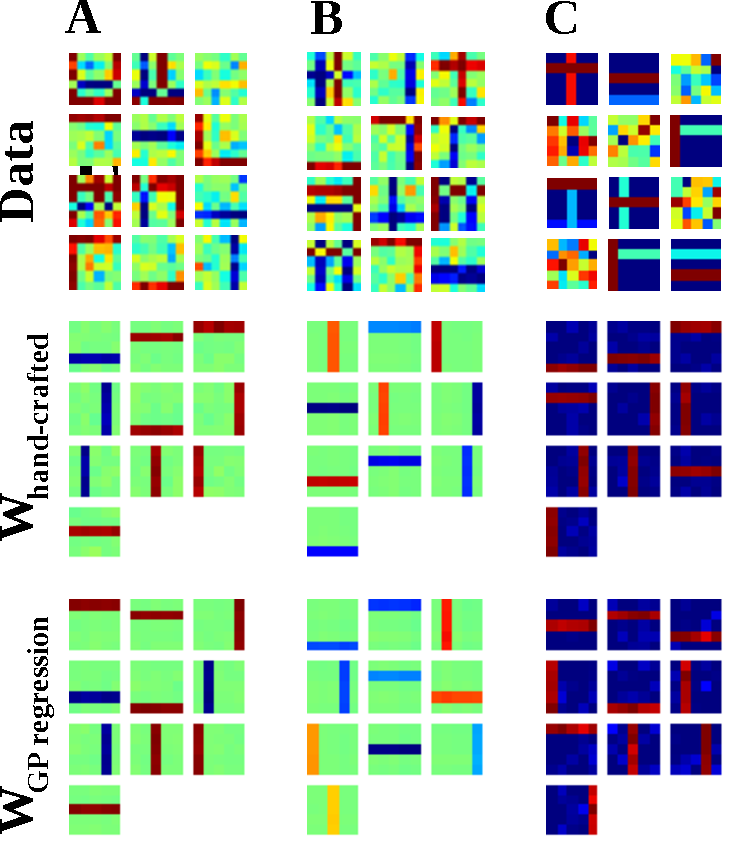
\includegraphics[width=.45\textwidth]{figs/sparsecoding/bars-test.pdf}
%\subfigure[Data and converged\\ solution]{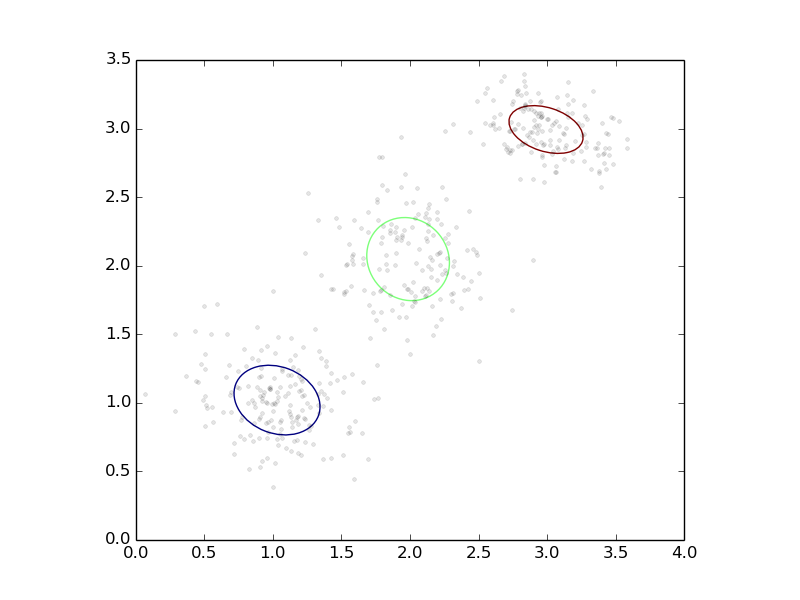
\includegraphics[width=.25\textwidth]{figs/mog/learn-rbf-h2/040.png}}
%\subfigure[GP regression\\ function]{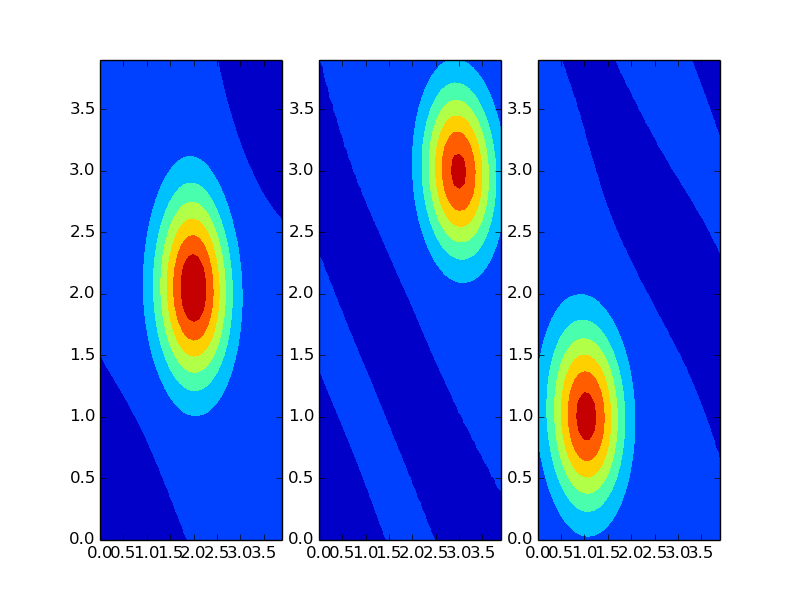
\includegraphics[width=.21\textwidth]{figs/mog/learn-rbf-h2/GP_pred_40.png}}\\
%\centerline{\fbox{This figure intentionally left non-blank}}
\caption{Sparse coding models results comparing GP-select with a successful hand-crafted selection function.
Results are shown on artificial ground-truth data with $H=10$ latent variables and $H'=5$ preselected variables for: \textbf{A} Binary sparse coding, \textbf{B} Spike-and-slab sparse coding, and \textbf{C} Nonlinear spike-and-slab sparse coding.
Top row: Example data points $\vec{y}^{(n)}$ generated by each of the models.
Middle row: Converged dictionary elements $W$ learned by the hand-crafted selection functions.
Bottom row: Converged dictionary elements $W$ learned by the GP-select with $H'=5$ using the kernel with best performance (matching that of inference with hand-crafted selection function).
}\label{fig:sparse}
\end{center}
\end{figure}

Results are shown in Figure~\ref{fig:sparse}.
In all experiments, the GP-selection approach could infer ground-truth parameters as well as the hand-crafted function.
For models where the cosine similarity was used (in (1) and (3)), GP regression with a linear kernel quickly learned the ground-truth parameters, and hence fewer iterations of EM were necessary.
In other words, even without providing GP-selection function explicit weights $W$ as necessary in the hand-crafted function, GP regression learned a similar enough function to quickly yield identical results.
Furthermore, in the model with a less straight-forward hand-crafted function (in the spike-and-slab model of (2)), only GP regression with an RBF kernel was able to recover ground-truth parameters.
In this case, (model (2)) GP-select using an RBF kernel recovered the ground-truth 'bars' in $7$ out of $10$ repetitions, whereas the hand-crafted function recovered the bases in $8$ instances.
The other models, algorithm using GP-select converged to the ground-truth parameters with the same average frequency as the hand-crafted functions.
%This suggests difficulty in predicting which kernel will work a priori.

%Hand crafted functions can do as well as exact case, as shown in papers.
%Some sort of kernel can do as well as a selection function engineered by hand.

% ------ FIXME -------- leave this??
Furthermore, as the composition kernel is flexible enough to adapt to both linear and nonlinear relationships, this supports it as a reasonable general choice.


\subsection{Gaussian mixture model}
%
Next, we apply GP-selection to a simple example, a Gaussian mixture model, where the flexibility of the approach can be easily and intuitively visualized.
%To illustrate the idea and benefit of this approach, we consider a simple motivating example: the problem setting posed by Gaussian mixture models.
The model of the observations is:
%
\vspace{-.2cm}
\begin{equation}\label{eq:mog}
p(\vec{y}^{(n)} | \mu_c, \sigma_c, \pi) = \sum_c^{C} \mathcal{N}(\vec{y}^{(n)}; \mu_c, \sigma_c) \, \pi_c
\end{equation}
%
where $C$ is the number of mixture components, the task is assign each data point to a cluster.
%%%  infer from which cluster each data point originates.
%%% The latent distribution gives the prior probability of a data point coming from each cluster $c$, $p(s^{(n)} = c | \pi) = \pi_c$, and data from the $c$th cluster are distributed according to the $c$th component, $p (\vec{y}^{(n)} | s^{(n)} = c) = p_c(\vec{y}^{(n)})$.
%%% Once a data point $\vec{y}^{(n)}$ is observed, the posterior probability distribution for the cluster it belongs to is
%%
%% \vspace{-.15cm}
%%\begin{equation}\label{eq:mog-post}
%% p(s^{(n)} = k | \vec{y}^{(n)}) = r_c^{(n)} = \frac{p_c(\vec{y}^{(n)})\, \pi c}{\sum_c^{C} p_c(\vec{y}^{(n)}) \, \pi c},
%% \end{equation}
%

The targets of the training data used for GP regression is cluster responsibilities for all data points, for $\mathcal{D} = \{ (y^{(n)}, \vec{r}^{(n)}) | n = 1, \dots, N \}$.
With this, we apply our GP-selection approach to this model, computing the selection function according to Equation~\eqref{eq:gp-sel-func} and following the approximate EM approach as in the previous experiments.
%%% by applying Equation~\eqref{eq:gp-sel-func} to compute the posterior distribution in~\eqref{eq:mog-post}.
%
%Although the increase in computational efficiency by selecting a reduced set of $K$ mixture components would only be e number of clusters considered to be in the data is very large,
% Depending on the data
In these experiments we consider three scenarios for EM learning of the data in Equation~\eqref{eq:mog}: GP-selection with an RBF covariance kernel and a linear covariance kernel.%, and the composition kernel used in the sparse coding experiments (RBF, linear, bias, and white).
%
%, where $r_c^{(n)}$ is the responsibility of the $k$th Gaussian for the $n$th data point, $y^{(n)}$.
%%% With this, we calculate the GP predictions following Equations~\eqref{eq:gp-sel-func} and use the prediction size to select which $c$ clusters to include in the normalization in the calculation of the responsibilities $\vec{r}$ (where $\vec{S}$ is substituted with $\vec{r}$).

For visualization purposes, we generate $2$-dimensional observed data ($\vec{y}^{(n)} \in \mathrm{R}^{D=2} $) from $C=3$ clusters -- first with randomly assigned cluster means, and second such that the means of the clusters lie roughly on a line.
In the GP-selection experiments, we select $C' = 2$ clusters to select from the full set (where $C'$ clusters is analogous to $H'$ latent variables in the non-mixture model setting),
%%% the indices for which are contained in $\mathcal{K}_n$),
and run $40$ EM iterations of the three experiments.
We randomly initialize the variance of the clusters $\vec{\sigma}_c$ and initialize the cluster means $\vec{\mu}_c$ at randomly selected data points.
Results are shown in Figure~\ref{fig:mog}.

\begin{figure*}[t]
\begin{center}
\includegraphics[width=.75\textwidth]{figs/mog/mog.pdf}
\caption{Gaussian mixture model results using GP-selection ($C'=2$) for inference.
Shown is the development of inference using \textbf{A} RBF covariance kernel in the regression, and \textbf{B} a linear covariance kernel.
For each iteration shown, we see (1) the observed data and their inferred cluster assignments and (2) the $C$ corresponding GP regression functions learned/used for GP-selection in that iteration. Different iterations are pictured due to different convergence rates. As shown, inference with GP-selection using a linear kernel is unable to assign the data points to the appropriate clusters, whereas GP-selection with an RBF kernel succeeds.}\label{fig:mog}% iterations RBF: 0, 1,, 20, LIN: 0,10, 20
\end{center}
\end{figure*}

%%% XXX NOT TRUE: When the data are allowed to have clusters with means scattered about, both kernels used for GP-selection inference can find the optimal cluster assignments of the data.
With cluster parameters initialized randomly on these data, the linear GP regression prediction cannot correctly assign the data to their clusters (as seen in Figure~\ref{fig:mog}\textbf{B}), but the nonlinear approach successfully and easily finds the ground-truth clusters (Figure~\ref{fig:mog}\textbf{A}).
Furthermore, even when both were initialized in the optimal solution, the cluster assignments from GP-selection with a linear kernel quickly wandered away from the optimal solution and was identical to random initialization, converging to the same result shown in iteration 20 of Figure~\ref{fig:mog}\textbf{B})
The RBF kernel cluster assignments remained in the optimal solution even with number of preselected clusters set to $C'=1$.

%%% These experiments demonstrate that inference using GP-selection can successfully infer ground-truth cluster assignments in a mixture model using both a linear and nonlinear covariance kernel in the GP regression.

These experiments demonstrate that, not only is it difficult to know the relationship of the inputs and the output variables a priori,
but the structure of the data strongly plays a role in the success of using selection in inference.
%which makes hanand which kernel to choose / which selection function would be the best.
%Moral of the story will be to throw a kernel that can handle nonlinearities.
%Thus, selecting the variables in a flexible and nonlinear can successfully do inference, when a linear selection would not.
Given one likely cannot know a priori the structure of the (potentially high-dimensional) data, these results suggest using a flexible kernel that can handle diverse data.


%%%As can be seen, if we observe data that truly originates from $\mathcal{N}(\mu_{1}, \sigma_{1})$, GP-selection will always predict the incorrect Gaussian, because $\mathcal{N}(\mu_{2}, \sigma_{2})$: $f_{2}(\{\vec{y}_n\}$ will always be larger than $f_{1}(\{\vec{y}_n\}$.
%
%%%The GP will always assign a higher predictive probability to the wrong class for data originating from the other.

%- choosing features, comp speed up, approximately solving regression (random features, subset of data points -- don't need super good regression solution to pick relevant features, only the size of the regression prediction) robustness/better optima
% sel-samp shown to work well in parallelized large scale setting
% this is preliminary work, believe it cold be very powerful in high-dimensional setting

\subsection{Translation Invariant Occlusive models}

\begin{figure*}[t]
\begin{center}
%\centering
%\begin{subfigure}[b]{.25\textwidth}
%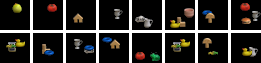
\includegraphics[width=\textwidth]{figs/inveca/dataSamples.png}
%\caption{}\label{fig:inveca_data}
%\end{subfigure}
%\begin{subfigure}[b]{.21\textwidth}
%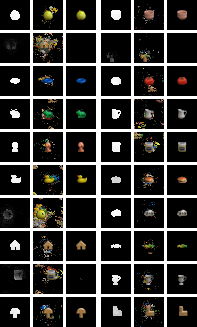
\includegraphics[width=\textwidth]{figs/inveca/params.png}
%\caption{}\label{fig:inveca_params}
%\end{subfigure}
%\\
%\begin{subfigure}[b]{.21\textwidth}
%\begin{center}
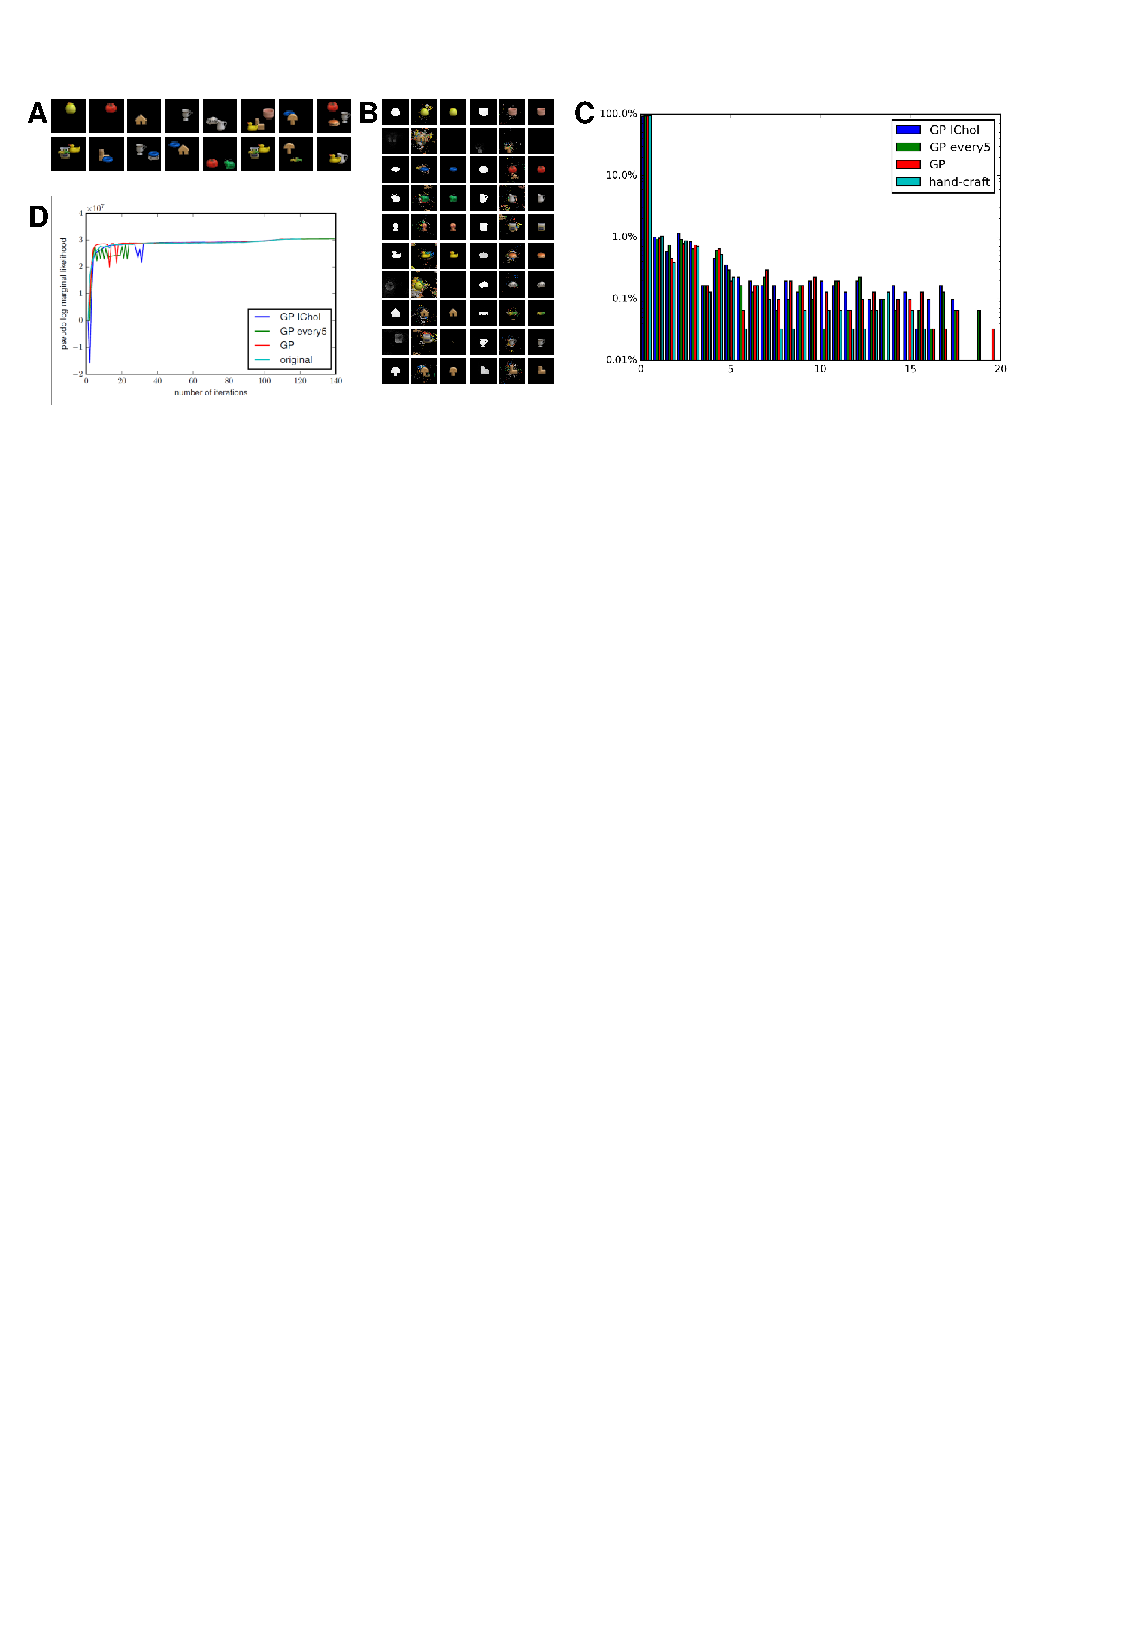
\includegraphics[width=\textwidth]{figs/inveca/invec.pdf}
%\caption{}\label{}%_locationhist}
%\end{subfigure}

%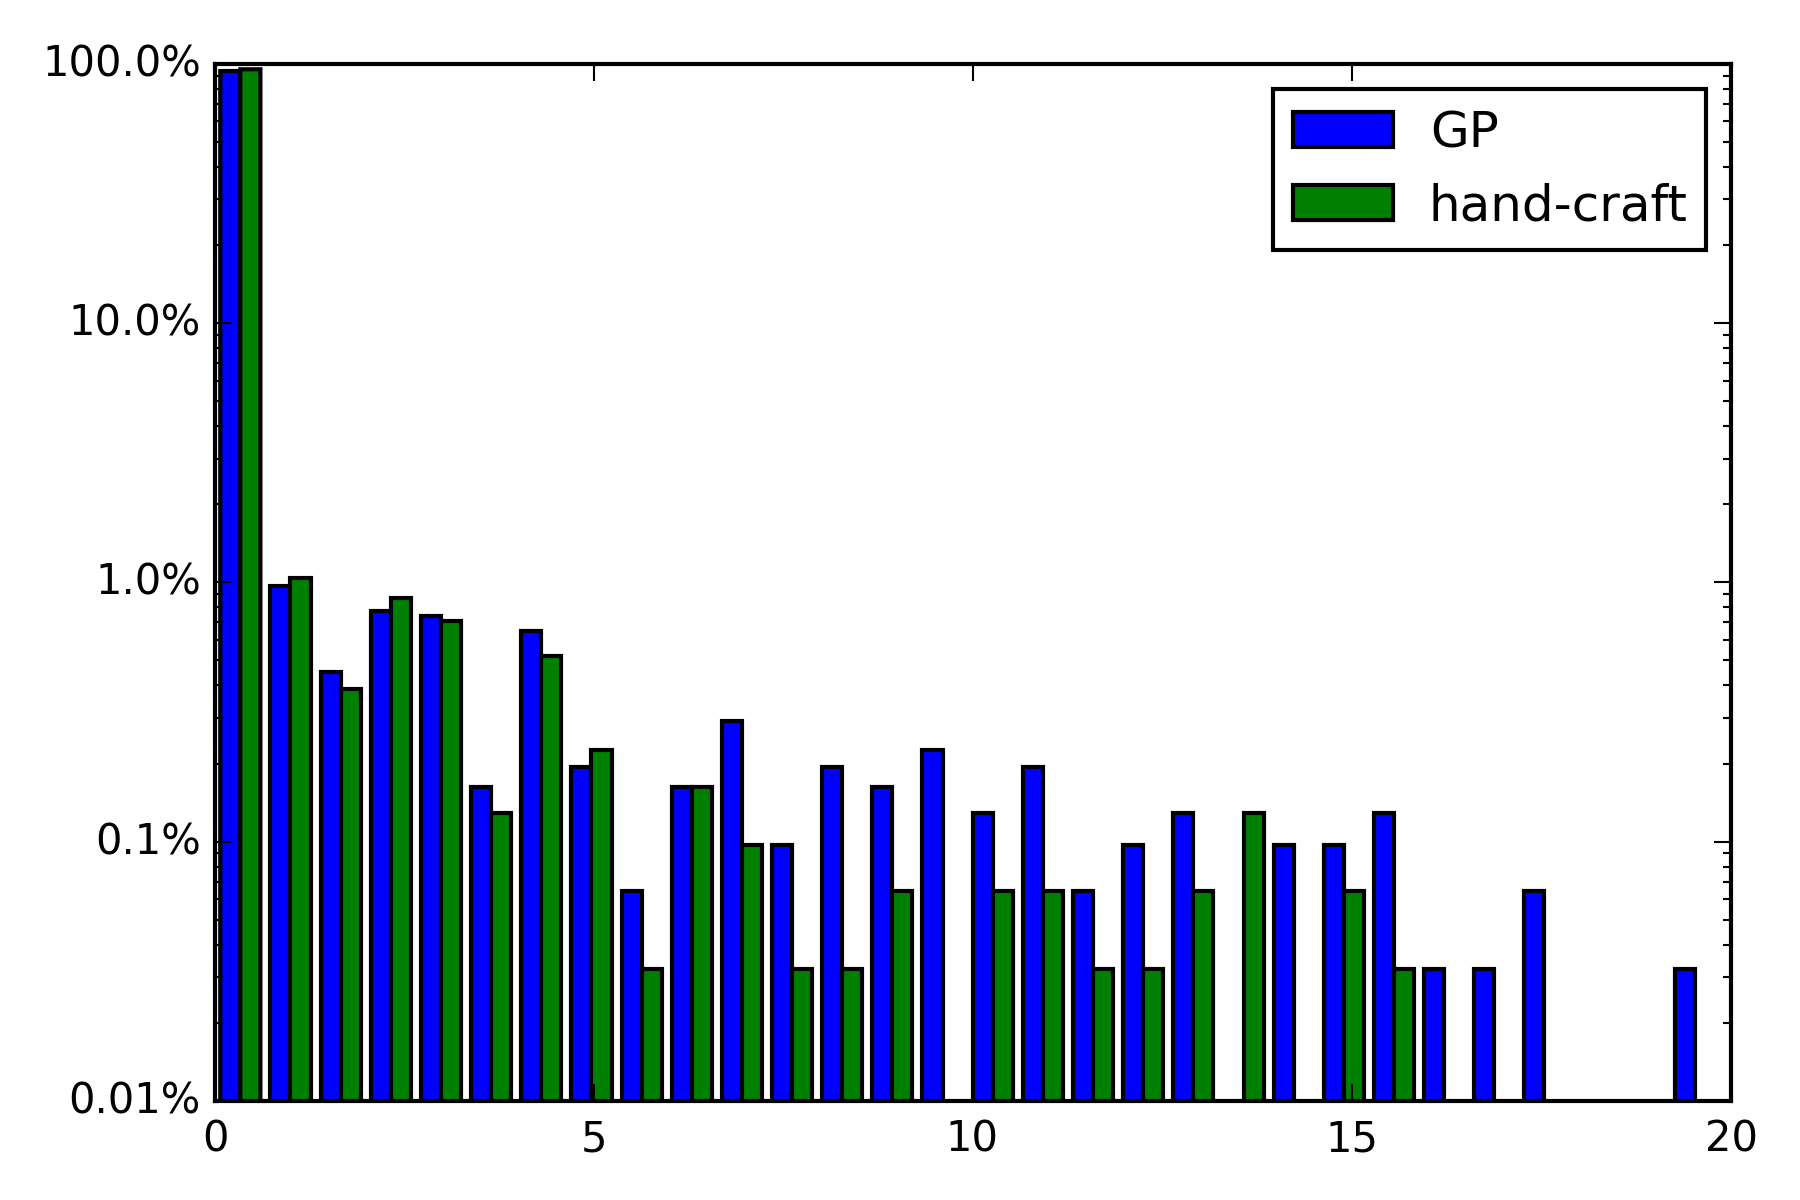
\includegraphics[width=\textwidth]{figs/inveca/locationHist.png}
\caption{Results of GP-select on the Translation Invariant model.
\textbf{A} shows some example from the dataset.
\textbf{B} shows the learned components and their masks. The first column shows the mask of each component, the second column shows the learned feature representations, and the third column only shows the area of the learned components with mask higher than $0.5$.
\textbf{C} shows the log-scale histogram of the prediction accuracy for both selection functions in terms of the distance from the predicted location to the ground truth location: the $x$-axis shows the distance from the ground-truth location in terms of pixels, and the $y$-axis shows the percentages.
\textbf{D} shows the convergence of the pseudo log-likelihood [of the model parameters learned at each EM iteration] for the both selection functions over all EM iterations. Figures \textbf{C} and \textbf{D} demonstrate the matching inference performance of both selection functions. % used for inference in this model: GP-select and the original hand-crafted one.
}
\label{fig:inveca}
\end{center}
\end{figure*}

Now that we have verified GP-select can be applied to diverse graphical models and converge to ground-truth parameters, we consider a more challenging model that addresses a problem in the computer vision domain.

Here we consider models that cope with translations of objects in a scene.
Such models are particularly difficult to optimize because they must consider multiple objects and locations in a scene -- the complexity of latent space becomes the number of locations exponentiated by the number of objects.
% --- Hand-crafted pre-selections have been successfully applied to translational invariant models.
%Especially considering multiple objects in a scene, the complexity of latent space becomes the number of locations to the power of the number of objects.
Inference in such a massive latent space heavily relies on the idea of variable selection to reduce the number of candidate objects and locations. In particular, hand-engineered pre-selection functions that consider translational invariance have been successfully applied to this type of model~\citep{DaiLucke2012b,DaiLucke2014,DaiEtAl2013}.
%
In such a model, the construction of a subset of latent space mainly consists of two steps: first, the candidate locations of all the objects in the model are predicted, and then a subset of candidate objects that might appear in the image are selected according to the predicted locations.  Next, the reduced subspace $\Kn$ is constructed according to the combinatorics of the different locations of all the candidate objects.
% --- Then the true posterior probabilities are estimated for this preselected latent subspace, while considering the posterior probabilities in the rest space to be zero.
The posterior distribution is then computed following Equation~\eqref{eq:sel-post}.

One limitation of such a hand-engineered system is that the selection function itself has parameters which need to be hand-tuned, e.g., the number of representative features.%, which leads to problems when this number is either too big or too small.
Second, this selection function needs to scan through the entire image at all possible locations, which is very costly for large-scale experiments.
%
%In this experiment, we follow a similar design to use a GP regression model as a general selection. Different from the applications in previous models,
In translation invariant models, instead of predicting the existence of a component, the selection function has to predict all possible locations a component could be.
To maximally exploit the capabilities of GP-selection function, we directly use the GP regression model to \textit{predict the possible locations} of a component \textit{without introducing any knowledge of translation invariance} into the selection function.
Therefore, the input to GP-selection function is the image to be inferred and the output is a score for each possible location of each component in the model.
For example, for learning $10$ components in a $D=30\times 30$ pixel image patch, the output dimensionality of GP-select is $9000$.
Although this initially seems a challenging computation for GP-selection, this is not the case given GP models scale linearly with output dimensionality.
As we will show in the following experiment, inference with the GP-selection function performs significantly faster than the original selection function used in previous works, because it does not need to explicitly scan through image.

Intuitively, using GP-select for this problem makes sense, as objects are typically not uniformly distributed in a scene and with limited  observations we often can give a good rough prediction of object locations.
Approaches such as data-driven location are based entirely on this idea, going further to convert a detection problem into an information retrieval problem, and recently achieving the state-of-art performance on object detection \citep{Rodriguez-SerranoL13}.



\textbf{COIL Data.}
We apply our GP-selection function to the Invariant Exclusive Component Analysis (InvECA) model~\citep{DaiEtAl2013}.
We consider an image dataset that is heavily used in the computer vision literature: data were generated using objects from the COIL-100 image dataset \citep{coil100}, taking $16$ different objects, downscaled to $D=10 \times 10$ pixels and segmented out from the black background.
A given image was generated by randomly selecting a subset of the $16$ objects, where each object has a probability of $0.2$ to appear.
The appearing objects were placed at random positions on a $30 \times 30$ black image.
When the objects overlap, they occlude each other with a different random depth order for each image.
In total, $N=2000$ images were generated in the dataset (examples shown in Figure~\ref{fig:inveca}\textbf{A}).

%We apply the model with GP selection function and seek to learn $20$ objects from the dataset.
%
For this experiment, the GP model parameters are optimized at the end of each EM iteration, using a maximum of $20$ gradient updates with L-BFGS.
All images in the training set are used and the marginal truncated posterior probabilities are denoted $p(l_h | \vec{y}^{(n)})$, where $l_h$ is the location of the $h$ component. The number of objects sought to be learned is $H=20$ and preselected objects was $H'=5$.

Results are shown in Figure~\ref{fig:inveca}.
GP-select successfully recovers all objects in the dataset, all of which are shown with their masks in Figure~\ref{fig:inveca}\textbf{B}.
Four additional components developed into representations, all of which have very low mask values,  which can easily tell from other true components.
In order to quantify the accuracy of our GP-selection function, we collected the GP-selection after learning, and applied the GP selection function to the whole dataset again, then compared with the ground-truth location of all the objects in the datasets.
%
Then, the accuracy of the predicted locations are estimated by computing the distance from the location of the top candidate and the ground-truth location.
These distances are plotted as a histogram in Figure~\ref{fig:inveca}\textbf{C}.
As a comparison, we also estimated the prediction accuracy of the original hand-craft selection function. Both selection functions can very accurately predict the locations of all the objects in the dataset.
Furthermore, the pseudo-log likelihood for both selection functions are shown in Figure~\ref{fig:inveca}\textbf{D}.
% FIXME TODO ---- pseudo like

Because GP selection avoids explicitly scanning through the whole image, the time of inference is significantly faster than the original selection function. For the GP-selection function, which was applied without any approximations or tricks to enhance speed, inferring the whole dataset (2000 images) required $22.1$ seconds on a single CPU core, while the inference with the original selection function required $1830.9$ seconds on a single CPU core.
In the original work, the hand-crafted selection function was implemented with GPU acceleration and parallelization.


% potential extension multiple output GP.
% cascade prediction

\section{Discussion}
%
% XXX changed score to selection
We have proposed a means of achieving fast EM inference in Bayesian generative models, by
learning an approximate selection function to determine relevant latent variables
for each observed variable. The process of learning the relevance functions
is interleaved with the EM steps, and these functions
are used in obtaining an approximate posterior distribution in the subsequent EM iteration.
The functions themselves are learned via Gaussian process regression,
and do not require domain-specific engineering, unlike previous regression functions.
In experiments on simple and easily interpretable models (spike-and-slab, Gaussian mixtures),
the learned selection functions behaved in accordance with our expectations for the posterior
distribution over the latents.  

The significant benefit we show empirically is that by learning the selection function in a general and flexible nonparametric way, we can avoid using expensive hand-engineered selection functions.
Cost reduction is both in terms of required expertise in the problem domain, and computation time in identifying the relevant latent variables.
Inference using our approach required 22.1 seconds on a single CPU core, versus  1830.9 seconds with the original hand-crafted function 
for the complex hierarchical model of \citep{DaiLucke2014}.


A major area where further performance gains might be expected is in
improving computational performance, since we expect the greatest
advantages of GP selection to occur for complex models at large scale. For instance,
 kernel ridge regression
may be parallelized \citep{zhang14divide},
or the problem may be solved in the primal via random Fourier features \citep{LeSarSmo13}.
Furthermore, there are many recent development regarding the scaling up of GP inference to large-scale problems, e.g., sparse GP approximation
~\citep{sparseGP}, stochastic variational inference \citep{HensmanEtAl2013,Hensman2012}, using parallelization techniques and GPU acceleration \citep{butt}.

\iffalse
\subsubsection*{Acknowledgements}
We acknowledge funding by the German Research Foundation (DFG) under grant LU 1196/4-2 (JS), by the Cluster of Excellence EXC 1077/1 "Hearing4all" (JL), and by the RADIANT and WYSIWYD (EU FP7-ICT) projects (ZD).
\fi

\bibliography{cnml-all.bib}
\bibliographystyle{icml2015}



% XXX
%The increase generality and flexibility of GP selection does not come without any cost, however.
%Depending on the used kernel, the computational demand for GP selection can scale polynomial with the number of data points (HI GUYS PLEASE VERIFY THIS and add if cubic or quadratically) while most previously used selection functions scale linearly. By coupling selection function learning to GPs, any improvements for GP inference and learning can directly be leveraged, however.
%Ongoing research for efficient GP classification investigates, for instance, NOW NAME APPROACHES HERE - ARTHUR, ZHENWEN?
%
%AG
%Furthermore, given complex graphical models, GP selection could be applied to help guide the design of more efficient but model specific selection functions, or to validate such functions. The experiments presented here could, for instance, also be interpreted as a validation of the selection functions used in previous work.
%
%Smaller-scale applications can be used for comparison of model specific selection functions and GP selection as discussed here; efficient model specific selection function defined using GPs could then be used for large-scale applications.

%Current work is applying the GP inference approach to complex models at large-scale, where we expect to the benefits of this approach to shine -- both in terms of computational efficiency as well as the flexibility offered by such a simple regression approach to "pre-learn" complicated inference landscapes.
% - approximate GP regression -- subset of data to compute kernel matrix?
% - low rank approx to kernel matrix?
% - optimize kernel parameters on a less-frequent schedule .. i.e. based on how much the parameters changed the last times it optimized
% - don't compute regression every EM iteration -- use the same regression from previous iterations when the predictive covariance is "low enough" ... but then "low enough" needs to be defined

% % OLD discussion
% Results so far are promising -- the Gaussian mixture model demonstrated that data exist for which a linear predictor will always fail at finding relevant features, whereas a nonlinear predictor offers flexibility without a priori assumptions.
% The results on diverse sparse coding models also demonstrate the power of the approach in its ability to learn selection functions
% hand-engineered selection functions even via simple linear regression.
% Current work is applying this inference approach to complex models at large-scale, where we expect to the benefits of this approach to shine -- both in terms of computational efficiency as well as the flexibility offered by such a simple regression approach to "pre-learn" complicated inference landscapes.
% Considering the translational invariant exclusive model, the pre-selection consists of two steps: first, selecting a small of candidate positions for each component in the model, and then selecting a small set of candidate components.

% The GP-selection approach lends itself to many possible ways of being applicable at larger scale, which is a topic of ongoing research. Mention ideas to scale up??
% - approximate GP regression -- subset of data to compute kernel matrix?
% - low rank approx to kernel matrix?
% - optimize kernel parameters on a less-frequent schedule .. i.e. based on how much the parameters changed the last times it optimized
% - don't compute regression every EM iteration -- use the same regression from previous iterations when the predictive covariance is "low enough" ... but then "low enough" needs to be defined
